\documentclass[10pt, letterpaper]{article}

%% Language and font encodings
\usepackage[english]{babel}
\usepackage[utf8x]{inputenc}
\usepackage[T1]{fontenc}

%% Sets page size and margins
\usepackage[a4paper, top=3cm, bottom=2cm, left=3cm, right=3cm, marginparwidth=1.75cm]{geometry}
\usepackage{caption, subcaption}
\captionsetup[table]{skip=10pt}

%% Useful packages
\usepackage{amsmath, graphicx, natbib, multicol, booktabs}
\usepackage[colorinlistoftodos]{todonotes}
\usepackage[colorlinks=true, allcolors=blue]{hyperref}
\bibliographystyle{unsrt}
%% Title
\title{
    \usefont{OT1}{bch}{b}{n}
    \normalfont \normalsize \textsc{STEM Fellowship Big Data Challenge 2020} \\ [10pt]
    \huge Deep learning transcriptomic model for prediction of pan-cancer chemotherapeutic sensitivity \\
}
\selectlanguage{english}
\usepackage{authblk}
\author[1]{Eddie Guo}
\author[2]{Mehul Gupta}
\author[1]{Pouria Torabi}
\author[2]{Sunand Kannappan}
\affil[1]{University of Alberta}
\affil[2]{University of Calgary}

% drawing neural network
\usepackage{tikz}
\usetikzlibrary{shapes, arrows}
\tikzset{
  every neuron/.style={
    circle,
    draw,
    minimum size=1cm
  },
  neuron missing/.style={
    draw=none, 
    scale=3,
    text height=0.333cm,
    execute at begin node=\color{black}$\vdots$
  },
}

\usepackage{ifthen}
\newcommand{\foo}[1]{%
  \ifthenelse{\equal{#1}{missing}}
    {}
    {\scriptsize $H^{(1)}_{\l}$}
}

\newcommand{\hehe}[1]{%
  \ifthenelse{\equal{#1}{missing}}
    {}
    {\scriptsize $H^{(2)}_{\l}$}
}

\newcommand{\hehetwo}[1]{%
  \ifthenelse{\equal{#1}{missing}}
    {}
    {\scriptsize $H^{(3)}_{\l}$}
}

\newcommand{\hehethree}[1]{%
  \ifthenelse{\equal{#1}{missing}}
    {}
    {\scriptsize $H^{(4)}_{\l}$}
}

\newcommand{\lmao}[1]{%
  \ifthenelse{\equal{#1}{missing}}
    {}
    {\scriptsize $I_{\l}$}
}

% define flowchart styles
\tikzstyle{block} = [rectangle, rounded corners, minimum height=4em, draw=black, inner sep=1em]
\tikzstyle[line] = [draw, -latex']
\tikzstyle{stop} = [rectangle, rounded corners, minimum width=2cm, minimum height=0.5cm,text centered, draw=black]
\tikzstyle{arrow} = [thick,->,>=stealth]

\frenchspacing


\begin{document}
\maketitle

\begin{multicols}{2}
% Abstract
\begin{abstract}
    [INSERT HERE]
\end{abstract} \vspace{1em}

% Keywords
\noindent {\textbf{Keywords}\\
neural network, pan-cancer, clustering}


% Introduction
\section{Introduction}
It is well established that tumour sensitivity to chemotherapy is highly heterogeneous between, but also within cancer types. Despite this, traditional treatment courses are largely standardized within specific cancer types. As such, a subset of cancer patients fails to respond to cancer type-specific chemotherapy while also carrying a large side effect burden from treatment. Given the significant impact of chemotherapy failure and associated toxicities, it is crucial to improve methods to select chemotherapies tailored for individual cancer patients.

Past precision oncology strategies have largely focused on utilizing tumour-specific characteristics, including genetic aberrations and expression profiles, to generate targeted therapies. Emerging precision oncology approaches have begun to utilize molecular profiling of tumours to better select existing chemotherapies predicted to have high potency. While most chemotherapies are non-targeted and have broad activity, there are molecular determinants of chemotherapeutic efficacy, including gene expression. It is well known that gene expression may mediate chemotherapeutic activity pathways. Cell line drug panels provide a novel data source to inform these studies, providing in-vitro cell line sensitivity with associated molecular profiling. These data sources allow for the identification of genetic predictors of drug sensitivity.

We postulate that a gene signature can predict chemotherapeutic response across cancer types. This study effectively clustered cell lines into chemotherapeutic response profiles, followed by the development of a neural net model that could stratify cell lines into these clusters utilizing mRNA expression molecular profiling.


% Materials and Methods
\section{Methods}

\subsection*{Pan-cancer therapeutic response cohorts}
To better understand the impact and predictive ability of transcriptomic dysregulation in chemotherapeutic response, a pan-cancer cohort of cell-line and associated therapeutic efficacy data were obtained from the Genomics of Drug Sensitivity in Cancer (GDSC). This data includes 1,110 cell lines from various different tumour types, and is thought to represent a relatively comprehensive pan-cancer dataset. In addition, the acquired dataset contained therapeutic efficacy information in the form of half-maximal inhibitory concentration (IC$_{50}$) values for 251 chemotherapies. These values correspond to the minimal concentration of therapeutic required to induce cell death in 50\% of the cells cultured, with lower values being associated with improved drug efficacy. This data was used to generate a matrix with cell-line and accompanying therapeutic information. This dataset was filtered to exclude therapies with less than 80\% of data for all cell-lines, followed by the exclusion of cell lines lacking response data for the drugs retained in the first step. This resulted in the inclusion of 548 cell-lines and 117 therapeutics for clustering based analysis.


\begin{figure*}[!ht]
    \centering
    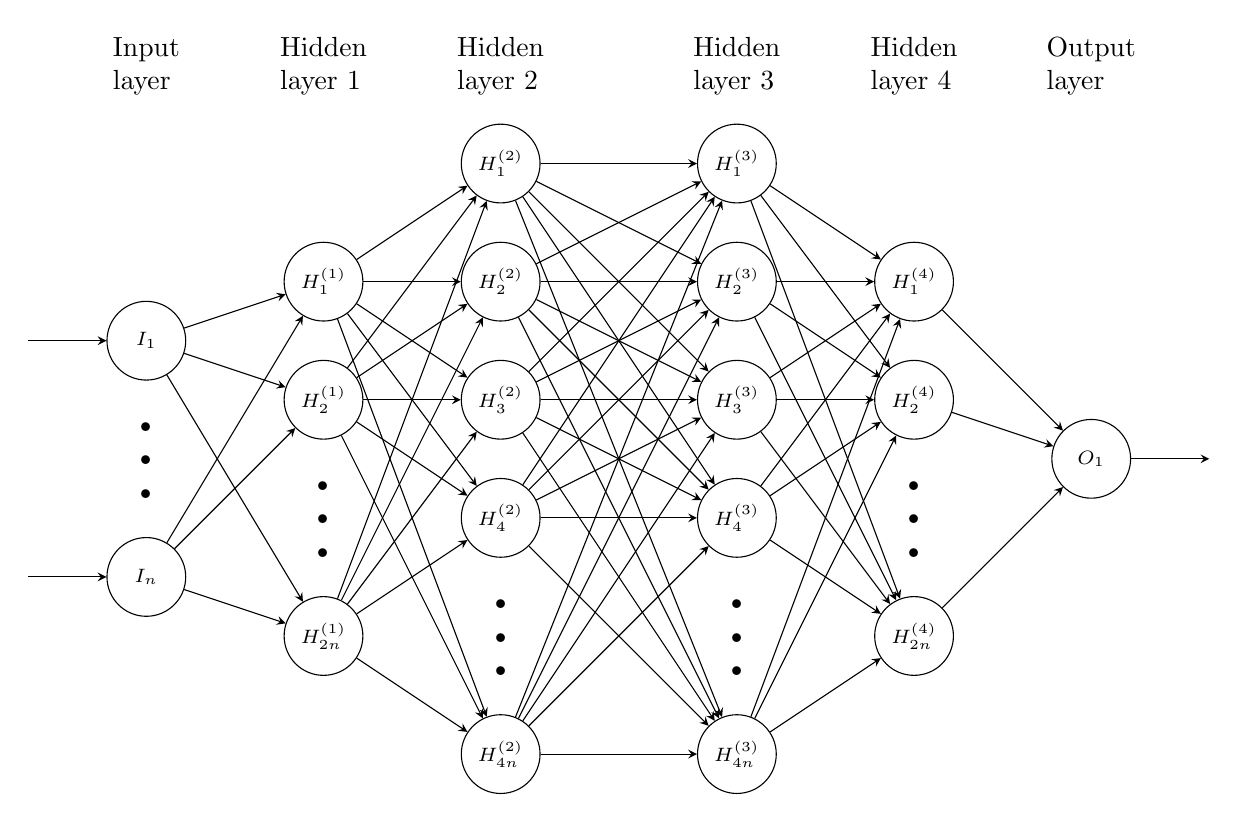
\begin{tikzpicture}[x=1.5cm, y=1.5cm, >=stealth]
    
        % nodes
        \foreach \m/\l [count=\y] in {1,missing,n}
            \node [every neuron/.try, neuron \m/.try] (input-\m) at (0,-1.5-\y) {\lmao{\l}};
        
        \foreach \m/\l [count=\y] in {1,2,missing,2n}
            \node [every neuron/.try, neuron \m/.try] (hidden-\m) at (1.5,-1-\y) {\foo{\l}};

        \foreach \m/\l [count=\y] in {1,2,3,4,missing,4n}
            \node [every neuron/.try, neuron \m/.try] (hidden1-\m) at (3,0-\y) {\hehe{\l}};
    
        \foreach \m/\l [count=\y] in {1,2,3,4,missing,4n}
            \node [every neuron/.try, neuron \m/.try] (hidden2-\m) at (5,0-\y) {\hehetwo{\l}};
    
        \foreach \m/\l [count=\y] in {1,2,missing,2n}
            \node [every neuron/.try, neuron \m/.try] (hidden3-\m) at (6.5,-1-\y) {\hehethree{\l}};
    
        \foreach \m/\l [count=\y] in {1}
            \node [every neuron/.try, neuron \m/.try] (output-\m) at (8,0-2.5-\y) {\scriptsize $O_1$};

        % arrows
        \foreach \l [count=\i] in {1,n}
            \draw [<-] (input-\l) -- ++(-1,0) node [above, midway] {};
    
        \foreach \l [count=\i] in {1,n}
            \foreach \k [count=\j] in {1,2,2n}
              \draw [->] (input-\l) -- (hidden-\k);
    
        \foreach \l [count=\i] in {1,2,2n}
            \foreach \k [count=\j] in {1,...,4,4n}
              \draw [->] (hidden-\l) -- (hidden1-\k);
    
        \foreach \l [count=\i] in {1,...,4,4n}
            \foreach \k [count=\j] in {1,...,4,4n}
              \draw [->] (hidden1-\l) -- (hidden2-\k);
    
        \foreach \l [count=\i] in {1,...,4,4n}
            \foreach \k [count=\j] in {1,2,2n}
              \draw [->] (hidden2-\l) -- (hidden3-\k);
    
        \foreach \l [count=\i] in {1,2,2n}
            \foreach \k [count=\j] in {1}
              \draw [->] (hidden3-\l) -- (output-\k);

        \foreach \l [count=\i] in {1}
            \draw [->] (output-\l) -- ++(+1,0) node [above, midway] {};

        % labelling layers
        \foreach \l [count=\x from 0] in {Input\\layer, Hidden\\layer 1, Hidden\\layer 2}
            \node [align=left, above] at (\x*1.5, -0.5) {\l};
        
        \node [align=left, above] at (5, -0.5) {Hidden\\layer 3};
        \node [align=left, above] at (6.5, -0.5) {Hidden\\layer 4};
        \node [align=left, above] at (8, -0.5) {Output\\layer};

    \end{tikzpicture}
    \caption{Neural network architecture representation with four hidden layers ($n=300$). Inputs include the feature-selected genes from the RNA-seq dataset. Each hidden layer has a dropout rate of 0.3 and is subject to batch normalization.}
    \label{fig:neural_vis}
\end{figure*}


\subsection*{Identification of pan-cancer therapeutic response cohorts}
Cell line therapeutic response matrices obtained from the GDSC consortium were used to bifurcate candidate cell lines into defined response cohorts. We developed a Euclidean distance matrix for the retained cell lines based upon their pan-chemotherapy response. This matrix was then used to identify an optimal number of clusters capable of representing the therapeutic heterogeneity identified across the cancer cell lines. K-means clustering was then utilized to assign cell line candidates to appropriate therapeutic response cohorts. Generalized differences in chemotherapeutic efficacy between cohorts were visualized using a heatmap generated by the Pheatmap package in R. Separation between clusters was also visualized using principal component analysis with the factoextra package in R. Following the identification of defined clusters, differences in therapeutic efficacy between the identified cohorts were evaluated. Mann-Whitney U tests were utilized to compare the half-maximal inhibitory concentration (IC50) values between the groups. False discovery rate (FDR) correction was utilized to correct for multiple comparisons.


\begin{figure*}[!ht]
    \centering
    \begin{subfigure}[t]{0.5\textwidth}
        \centering
        \includegraphics[height=2.75in]{Figures/pca.png}
        \caption{}
        \label{fig:pca}
    \end{subfigure}%
    ~
    \begin{subfigure}[t]{0.5\textwidth}
        \centering
        \includegraphics[height=2.75in]{Figures/volcano.png}
        \caption{}
        \label{fig:volcano}
    \end{subfigure}

    \begin{subfigure}[t]{\textwidth}
        \centering
        \includegraphics[width=\textwidth]{Figures/heatmap.png}
        \caption{}
        \label{fig:heatmap}
    \end{subfigure}

    \caption{(\ref{fig:pca}) Principal component analysis of cell line therapeutic efficacy. The two identified therapeutic response clusters are indicated in blue and red respectively. (\ref{fig:volcano}) Volcano plot identifying chemotherapeutics with significantly different IC50 values between therapeutic response clusters. Drugs identified in red meet the criteria for significance (FDR adjusted $p<0.05$). (\ref{fig:heatmap}) Heatmap of therapeutic IC$_{50}$ for the two identified therapeutic response clusters. Columns represent individual chemotherapies, and are clustered according to Euclidean distance. Colours range from yellow to purple, with a shift toward the latter indicating increased efficacy of the corresponding chemotherapeutic.}
    \label{fig:clustering}
\end{figure*}


\subsection*{Feature Selection}
Feature reduction was the first of multiple steps taken to avoid overfitting. The number of genes within the RNA-seq dataset were reduced using the BorutaPy package in Python 3. The Boruta algorithm is a feature selection wrapper algorithm based on Random Forest classification, and it iteratively removes features that are statistically less significant than a shuffled version of the same feature. The algorithm identified 300 relevant genes from the original set of 16,382 genes at $\alpha=0.05$ with a maximum tree depth of 5. Given the feature variance in RNA expression, prior to fitting the model, expression values were scaled by z-score.


\begin{figure*}[!ht]
    \centering
    \begin{subfigure}[t]{\textwidth}
        \centering
        \includegraphics[width=\textwidth]{Figures/confusion_matrix/cm_combined.png}
        \caption{}
        \label{fig:cms}
    \end{subfigure}

    \begin{subfigure}[t]{\textwidth}
        \centering
        \includegraphics[width=\textwidth]{Figures/roc/full_merged.png}
        \caption{}
        \label{fig:roc}
    \end{subfigure}

    \caption{(\ref{fig:cms}) From left to right: confusion matrices for the 3, 4, and 5 hidden layer neural network models evaluating the true positive, false positive, true negative, and false negative rate. The models classify patient RNA-seq datasets into chemotherapy response cohorts. (\ref{fig:roc}) ROC curves for 3, 4, and 5 hidden layers neural network models with confidence bands of $\pm 1$ standard deviation. The models classify patient RNA-seq datasets into chemotherapy response cohorts. Each model was subject to 5-fold cross-validation and the mean across all trials was plotted.}
\end{figure*}



\subsection*{Classification using an optimized neural network}
The neural net was constructed using the Tensorflow Keras sequential deep learning API in Python 3. The model underwent multiple instances of optimization, starting with the manipulation of the overall hidden layer architecture. The classifier’s predictive accuracy and misclassification rate were monitored to determine the optimal number of dense hidden layers (Figure - confusion matrix) in addition to iterative manipulation of the number of neurons in each hidden layer. The rectified linear unit (ReLu) was chosen as the neuronal activation function for all the layers except the output layer which used a sigmoid activation as a means of classifying instances into binary classes. All optimization procedures were conducted on 80\% of the data, while the other 20\% was saved for model validation.

The model was rigorously monitored for and protected against overfitting. The dataset was randomly segregated into 80\% training and 20\% validation blocks. Additionally, dropout layers with a 0.3 dropout rate and batch normalization layers were employed to improve the generalizability of the model. Model selection was performed by tuning the model’s hyperparameters via a grid search and 5-fold cross-validation (Table \ref{tab:params}). We performed a grid search with 3-fold cross-validation on the training data (80\% of the dataset; 432 training samples, 541 overall) to determine the parameters under which to minimize the binary cross-entropy loss function. GridSearchCV from the scikit-learn library was used as a means of iterating through multiple possibilities of epochs, batch size, optimizer, and kernel initializer to find the optimal model. To prevent class imbalance during training, we used the Synthetic Minority Oversampling Technique (SMOTE) from the imblearn package for Python 3. Each model’s performance was evaluated by the area under the receiver operating characteristic (ROC) curve (AUC). Performance evaluation of the final model was performed with the testing set.


\begin{figure*}[!ht]
    \centering
    \includegraphics[width=\textwidth]{Figures/kegg.png}
    \caption{KEGG pathway functional enrichment for predictive genes included in the deep learning model conducted using g:Profiler.}
    \label{fig:kegg}
\end{figure*}



% Results
\section{Results}

\subsection*{Clustering of pan-cancer cell lines identifies two distinct therapeutic response cohorts}
To identify defined cohorts of pan-cancer cell-lines with similar trends in therapeutic efficacy, we employed clustering of retained cell-lines. This process identified two distinct clusters of therapeutic efficacy (Fig. \ref{fig:pca}), 362 cell lines identified in response group 1, and 186 cell lines identified in response group 2.  Further analysis of these clusters demonstrate that a subset of therapeutics performs substantially differently between the different cohorts (Fig. \ref{fig:heatmap}). To quantify differences in therapeutic response between clusters, IC50 values were compared between candidate cell lines (Fig. \ref{fig:volcano}). Of the 117 therapies included, 95 had significant differences in efficacy between the two cohorts identified. This suggests that these cohorts represent groups of cell lines with vastly different therapeutic responses. Therefore the ability to accurately stratify into these cohorts may be a valuable tool for stratification prior to chemotherapeutic treatment.

\subsection*{A neural network with four hiddeen layers accurately classifies patients into responder and non-respondeer cohorts}
Unsupervised learning in the form of the K-Means Clustering of the cancer cell line transcriptomes indicated substantially different responses to chemotherapies. Using these distinct therapy response cohorts, we developed a deep learning binary classification to predict drug response based on transcriptome data. We initially analyzed five neural network architectures, each corresponding to 1-5 hidden layers (Fig. \ref{fig:neural_vis}). Hyperparameter optimization via grid search returned similar results for each model: 50 epochs, batch size of 32, Adagrad as the optimizer, and a normal kernel initializer. Neural network architectures containing 3-5 hidden layers performed similarly with approximately 90\% accuracy. The architectures with 1 and 2 hidden layers performed less optimally with ~80\% accuracy. We proceeded to validate the architectures with 3-5 hidden layers using 5-fold cross-validation. Of note, the model with 4 hidden layers had the lowest false positive rate (FPR = 3.67\%) and a false negative rate (FNR = 4.59\%). The model with five hidden layers had the highest FPR of the models evaluated (8.26\%).

A receiver operating characteristic (ROC) curve was plotted for each of the neural network variants as an alternative evaluative method under uneven class sizes (Fig. \ref{fig:roc}). The relative ratio between the model’s false positive classification rate and its true positive rate was averaged between 5 K-Folds. The mean Area Under Curve (AUC) for the 5 trials was used to compare the three network architectures. However, the differences between the various architectures for AUC was not significatly different. Consequently, confusion matrices (Fig. \ref{fig:cms}) and associated misclassification rates were used to pick the optimal model. The neural net with 4 hidden layers boasted the best performance overall with a 91.7\% accuracy and an 8.3\% misclassification rate.


% Discussion
\section{Discussion}
In this study we developed an accurate deep learning-based model for classifying cancer patients based on RNA expression data into therapeutic response cohorts on a relatively small cell line therapeutic response dataset. Using unsupervised clustering techniques, we segregated cancer patients into two defined therapeutic response groups with significantly different responses to a multitude to standard chemotherapies. [EXPAND HERE]

The relatively low accuracy of the neural networks with 1 and 2 hidden layers (82.6\% and 70.8\% respectively) suggests that the therapeutic response cohorts cannot be separated by a linear classifier. Furthermore, the high FNR of the network with 5 hidden layers as compared to the 3 and 4 hidden layer networks indicates overfitting. To this end, either a 3 or 4 hidden layer network is the ideal architecture for analyzing our data. Interestingly, there is no significant difference between AUC for these models (Fig. \ref{fig:roc}). [EXPAND HERE]

A major limitation of our study was the availability of large datasets to train our model. Here we faced a $p$ $\gg$ $n$ problem as machine learning models expect that the number of features $p$ is much larger than the number of observations $n$. To minimize this bias, we applied the Boruta algorithm to reduce our 16,382 genes by 541 cell lines dataset to a 301 by 541 matrix. The algorithm has been shown in various journals to be an effective feature selector method in high dimensional omics datasets \cite{boruta}. To prevent overfitting of the reduced matrix, we applied batch normalization and dropout layers immediately preceding each hidden layer. Of note, a neural network architecture where the initial hidden layers diverge and the latter hidden layers converge provides the most accurate classifications of the RNA-seq data.

Future investigations will look to validate the efficacy of the model in prediction of chemotherapy response in various forms of cancer using the current transcriptomic signature. It is likely that the model accuracy will vary between therapy targets, as such, further studies can make use of our project pipeline to create a stratified model whereby the drug class and target are additional inputs.



% Conclusions
\section*{Conclusions}
Using transcriptomics data from the cancer cell lines, two chemotherapeutic response clusters were identified via unsupervised learning in the form of K-means Clustering. A feature selection algorithm was used to select a 300 gene signature which served as inputs to multiple neural networks. We determined that the network with 4 hidden layers was the most accurate model, producing a binary classifier to predict patient therapy response with 91.7\% accuracy.


% Acknowledgements
\section*{Acknowledgements}
INSERT HERE


\bibliography{bibliography}

\end{multicols}



\clearpage

\section*{Supplementary Data}
\subsection*{Figures}
\begin{figure}[!ht]
    \centering
    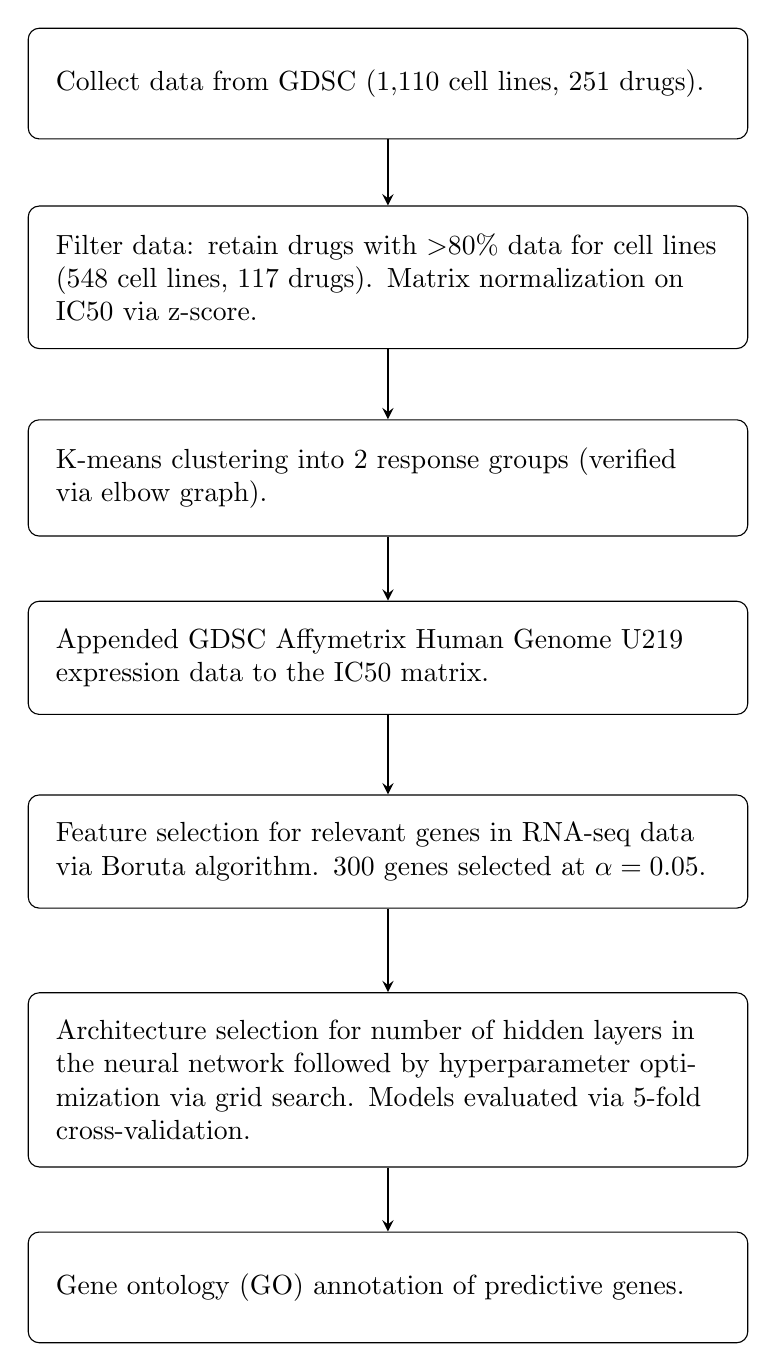
\begin{tikzpicture}[node distance=6em, auto]
        % blocks
        \node [block, text width=24em] (init) {Collect data from GDSC (1,110 cell lines, 251 drugs).};
        \node [block, below of=init, text width=24em, yshift=-1em] (process) {Filter data: retain drugs with $>$80\% data for cell lines (548 cell lines, 117 drugs). Matrix normalization on IC50 via z-score.};
        \node [block, below of=process, text width=24em, yshift=-1.25em] (kmeans) {K-means clustering into 2 response groups (verified via elbow graph).};
        \node [block, below of=kmeans, text width=24em, yshift=-0.5em] (append) {Appended GDSC Affymetrix Human Genome U219 expression data to the IC50 matrix.};
        \node [block, below of=append, text width=24em, yshift=-1em] (feat) {Feature selection for relevant genes in RNA-seq data via Boruta algorithm. 300 genes selected at $\alpha=0.05$.};
        \node [block, below of=feat, text width=24em, yshift=-2.25em] (neural) {Architecture selection for number of hidden layers in the neural network followed by hyperparameter optimization via grid search. Models evaluated via 5-fold cross-validation.};
        \node [block, below of=neural, text width=24em, yshift=-1.5em] (annot) {Gene ontology (GO) annotation of predictive genes.};

        % arrows
        \draw [arrow] (init) -- (process);
        \draw [arrow] (process) -- (kmeans);
        \draw [arrow] (kmeans) -- (append);
        \draw [arrow] (append) -- (feat);
        \draw [arrow] (feat) -- (neural);
        \draw [arrow] (neural) -- (annot);
    \end{tikzpicture}
    \label{fig:pipeline}
    \caption{Summary of the data analysis pipeline.}
\end{figure}

\clearpage

\subsection*{Tables}
\begin{table*}[!ht]
    \centering
    \caption{Grid search parameters to optimize all neural network architectures presented in this paper (3, 4, and 5 hidden layers). Each grid search underwent 3-fold cross-validation on the training data.}
    \label{tab:params}
    \begin{tabular}{l l l l}
        \toprule
        Epochs & Batches & Optimizer & Kernel initializer \\
        \midrule
        25 & 15 & Stochastic gradient descent & Normal \\
        50 & 32 & Adagrad & Uniform \\
        75 & 64 & Adam & Glorot uniform \\
        \bottomrule
    \end{tabular}
\end{table*}


\end{document}
